%%%%%%%%%%%%%%%%%%%%%%%%%%%%%%%%%%%%%%%%%
% Beamer Presentation
% LaTeX Template
% Version 1.0 (10/11/12)
%
% This template has been downloaded from:
% http://www.LaTeXTemplates.com
%
% License:
% CC BY-NC-SA 3.0 (http://creativecommons.org/licenses/by-nc-sa/3.0/)
%
%%%%%%%%%%%%%%%%%%%%%%%%%%%%%%%%%%%%%%%%%

%----------------------------------------------------------------------------------------
%	PACKAGES AND THEMES
%----------------------------------------------------------------------------------------

\documentclass{beamer}

\mode<presentation> {

% The Beamer class comes with a number of default slide themes
% which change the colors and layouts of slides. Below this is a list
% of all the themes, uncomment each in turn to see what they look like.

%\usetheme{default}
%\usetheme{AnnArbor}
%\usetheme{Antibes}
%\usetheme{Bergen}
%\usetheme{Berkeley}
%\usetheme{Berlin}
%\usetheme{Boadilla}
% \usetheme{CambridgeUS}
%\usetheme{Copenhagen}
%\usetheme{Darmstadt}
%\usetheme{Dresden}
%\usetheme{Frankfurt}
%\usetheme{Goettingen}
%\usetheme{Hannover}
%\usetheme{Ilmenau}
%\usetheme{JuanLesPins}
%\usetheme{Luebeck}
\usetheme{Madrid}
%\usetheme{Malmoe}
%\usetheme{Marburg}
%\usetheme{Montpellier}
% \usetheme{PaloAlto}
%\usetheme{Pittsburgh}
%\usetheme{Rochester}
%\usetheme{Singapore}
%\usetheme{Szeged}
%\usetheme{Warsaw}

% As well as themes, the Beamer class has a number of color themes
% for any slide theme. Uncomment each of these in turn to see how it
% changes the colors of your current slide theme.

%\usecolortheme{albatross}
%\usecolortheme{beaver}
%\usecolortheme{beetle}
%\usecolortheme{crane}
%\usecolortheme{dolphin}
%\usecolortheme{dove}
%\usecolortheme{fly}
%\usecolortheme{lily}
%\usecolortheme{orchid}
\usecolortheme{rose}
%\usecolortheme{seagull}
%\usecolortheme{seahorse}
%\usecolortheme{whale}
%\usecolortheme{wolverine}

%\setbeamertemplate{footline} % To remove the footer line in all slides uncomment this line
%\setbeamertemplate{footline}[page number] % To replace the footer line in all slides with a simple slide count uncomment this line

%\setbeamertemplate{navigation symbols}{} % To remove the navigation symbols from the bottom of all slides uncomment this line
}

\usepackage{graphicx} % Allows including images
\graphicspath{{./fig/}}
\DeclareGraphicsExtensions{.pdf,.jpeg,.png}
\usepackage{booktabs} % Allows the use of \toprule, \midrule and \bottomrule in tables
\usepackage[numberedbib]{apacite}

%----------------------------------------------------------------------------------------
%	TITLE PAGE
%----------------------------------------------------------------------------------------

\title[Auto Robot Arch: AI-perspective]
{Intro to Autonomous Robot Architecture: \\ From Artificial-intelligence Perspective \\
\vspace{5mm}
(Robotics Workshop, Computer Science, UI)
}

\author{Vektor Dewanto} % Your name
\institute[None] % Your institution as it will appear on the bottom of every slide, may be shorthand to save space
{
Affiliation: None\\ % Your institution for the title page
\medskip
\textit{vektor.dewanto@gmail.com } % Your email address
}
\date{\today} % Date, can be changed to a custom date

\begin{document}

\begin{frame}
\titlepage % Print the title page as the first slide
\end{frame}

\begin{frame}
\frametitle{Outline} % Table of contents slide, comment this block out to remove it
\tableofcontents % Throughout your presentation, if you choose to use \section{} and \subsection{} commands, these will automatically be printed on this slide as an overview of your presentation
\end{frame}

%----------------------------------------------------------------------------------------
%	PRESENTATION SLIDES
%----------------------------------------------------------------------------------------
%%%%%%%%%%%%%%%%%%%%%%%%%%%%%%%%%%%%%%%%%%%%%%%%%%%%%%%%%%%%%%%%%%%%%%%%%%%%%%%
\section{Introduction}
\frame{\tableofcontents[currentsection, hideothersubsections]}

\begin{frame}
\frametitle{Introduction}

\begin{figure}
    \centering
    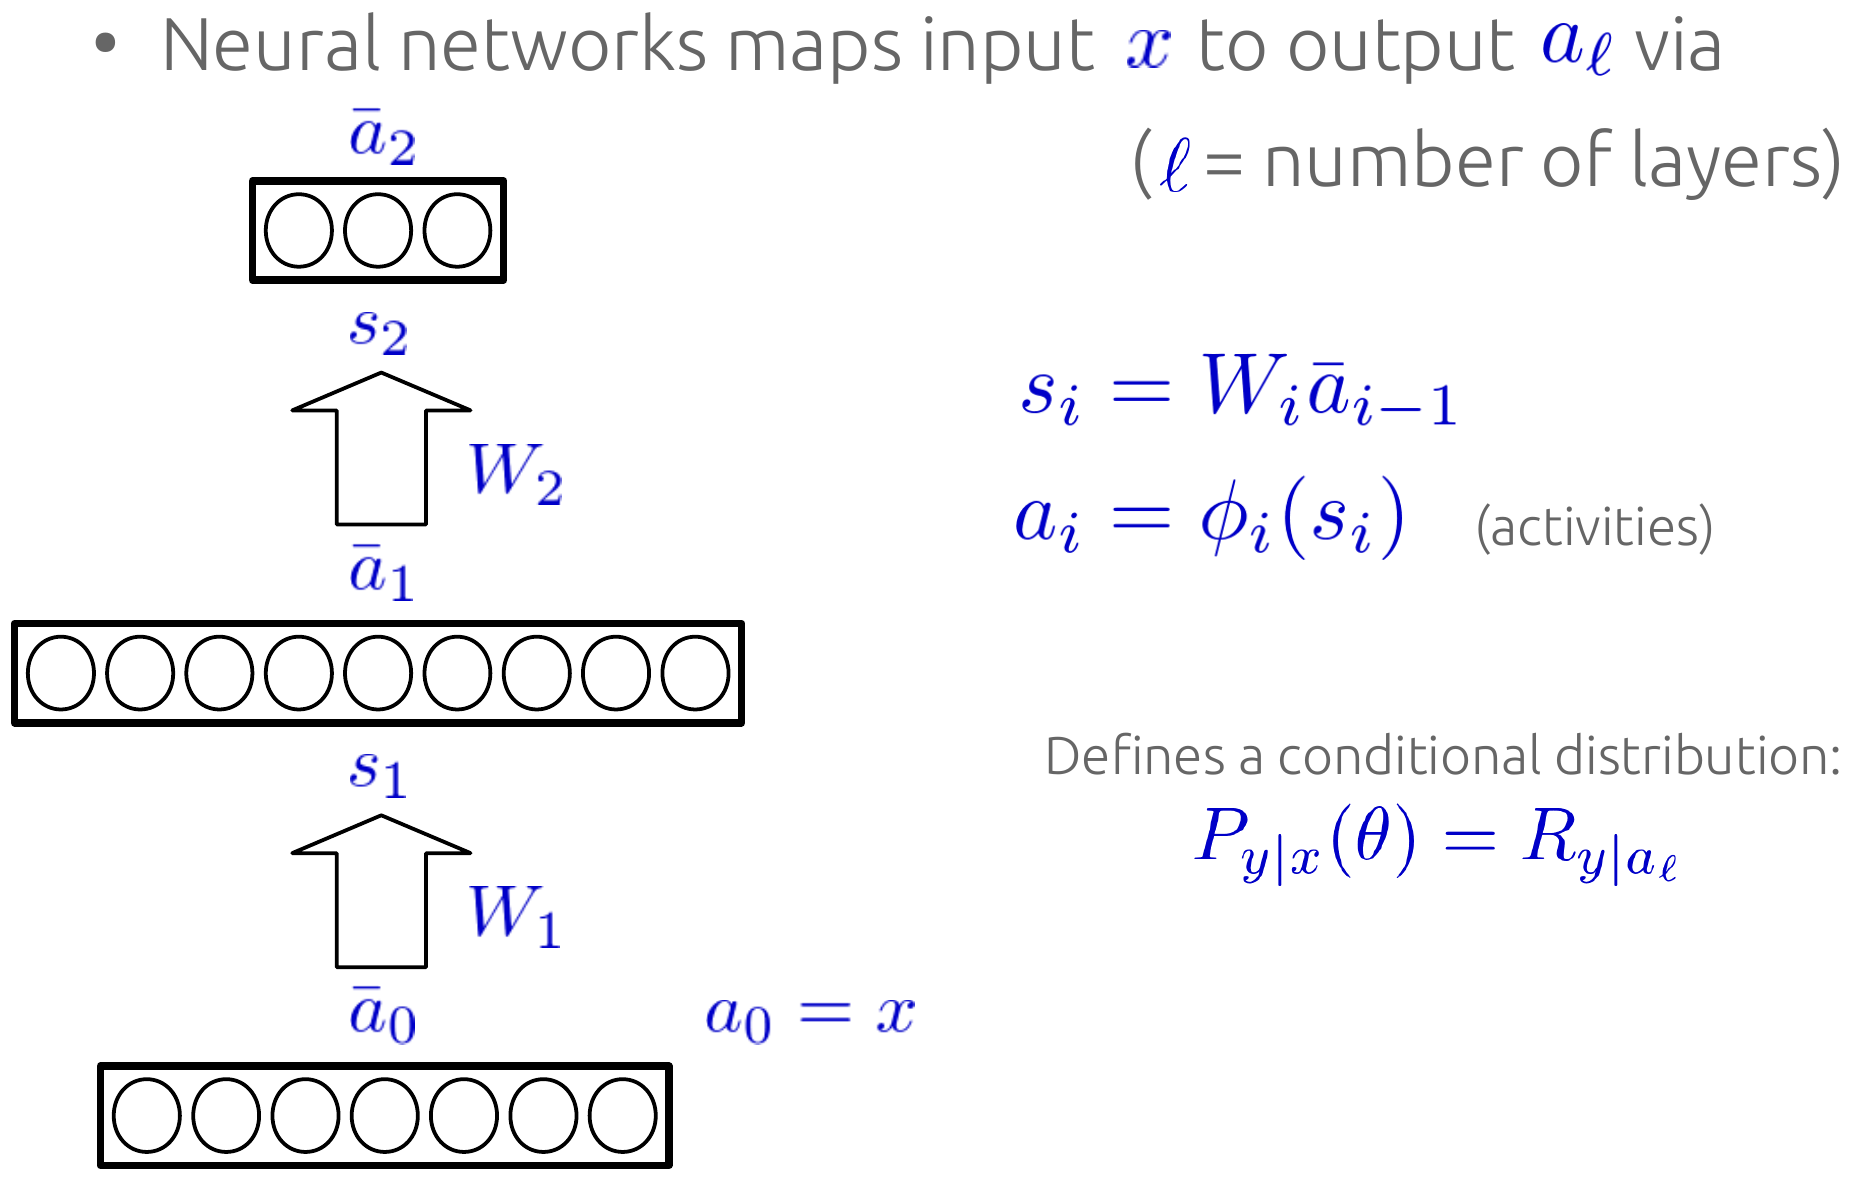
\includegraphics[scale=0.2]{net}
\end{figure}

\begin{itemize}
    \item $\bar{a}_i$ is $a_i$ appended by a homogeneous coordinate with value 1, ie
            to capture bias parameters explicitly
\end{itemize}
\end{frame}

\begin{frame}
\frametitle{Introduction}

\begin{figure}
    \centering
    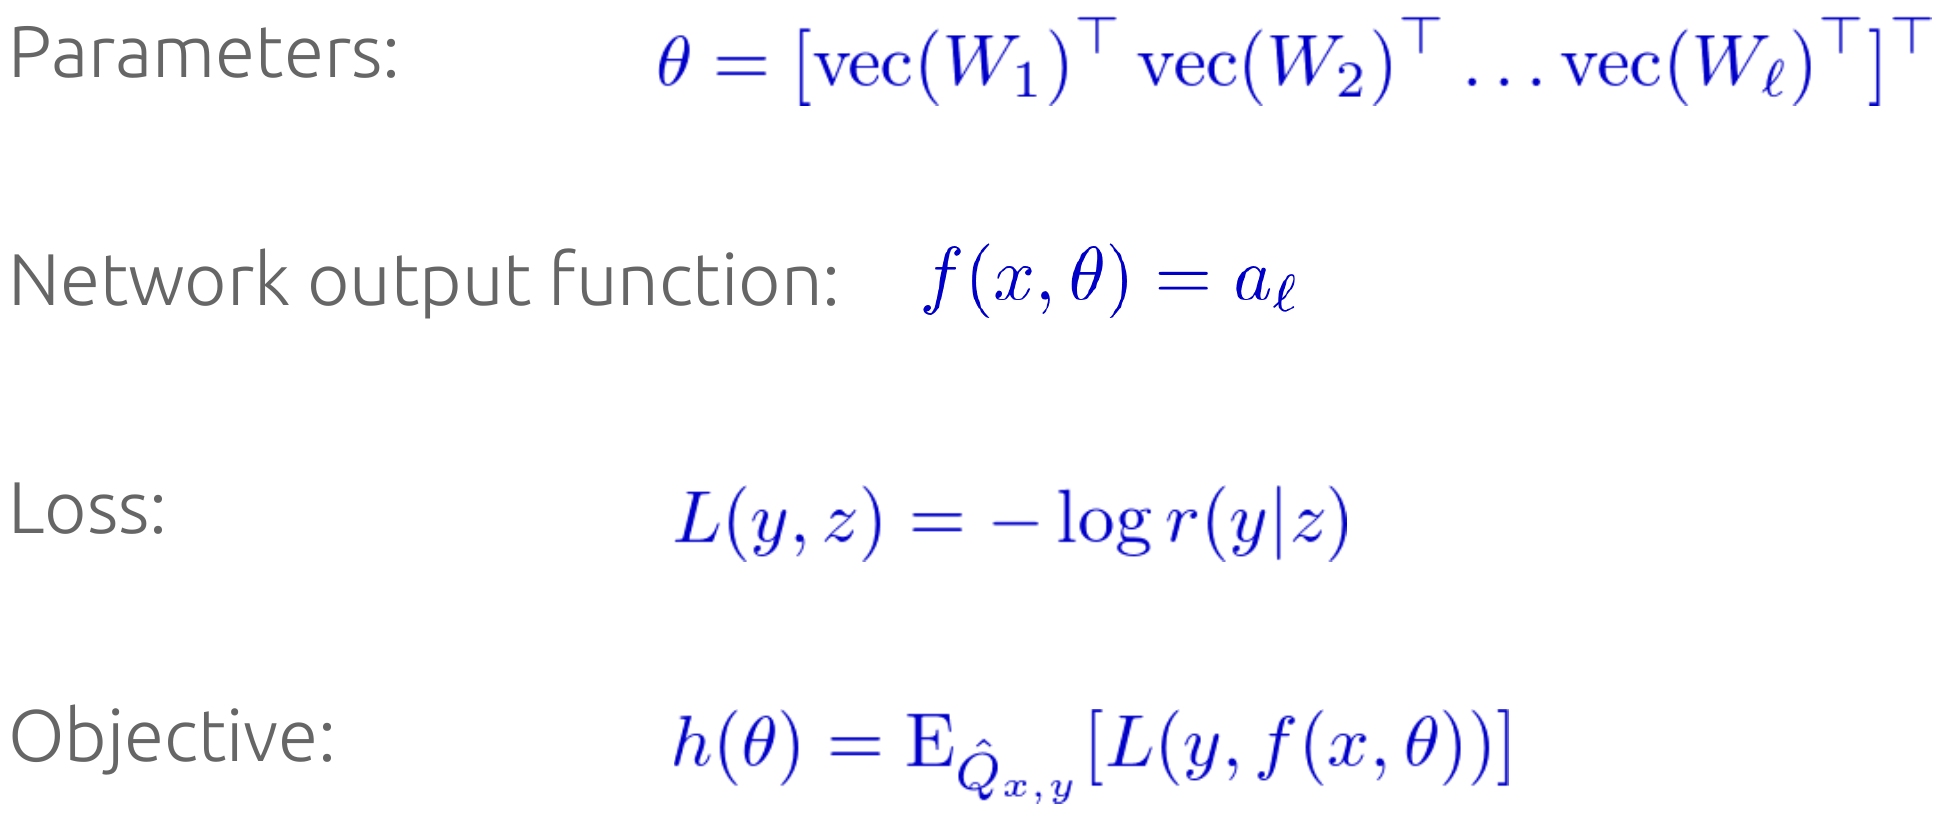
\includegraphics[scale=0.2]{net_param}
\end{figure}

\begin{itemize}
    \item $vec$ vectorizes matrices by stacking their columns together
    \item $\hat{Q}_{x, y}$ is a training distribution
    \item $p(y|x, \theta) = r(y|f(x, \theta))$ is the density function of $P_{y|x}(\theta) = R_{y|f(x,\theta)}$
    \item minimizing $h(\theta)$ can be seen as maximum likelihood learning of~$P_{y|x}(\theta)$.
\end{itemize}

\end{frame}

\begin{frame}
\frametitle{Introduction}
Newton-type update: $\theta_{k+1} = \theta_k - \alpha_k (\nabla^2 h)^{-1} \nabla h$
% \begin{itemize}
%     \item Newton-type update: $\theta_{t+1} = \theta_t - \alpha (\nabla^2 h)^{-1} \nabla h$
% \end{itemize}
\begin{figure}
    \raggedright
    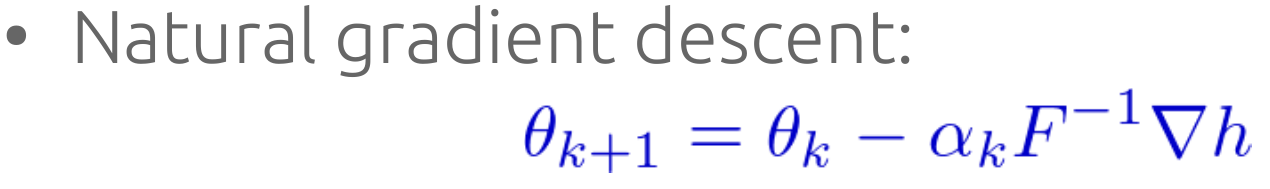
\includegraphics[scale=0.25]{natgrad}
\end{figure}

\begin{figure}
    \raggedright
    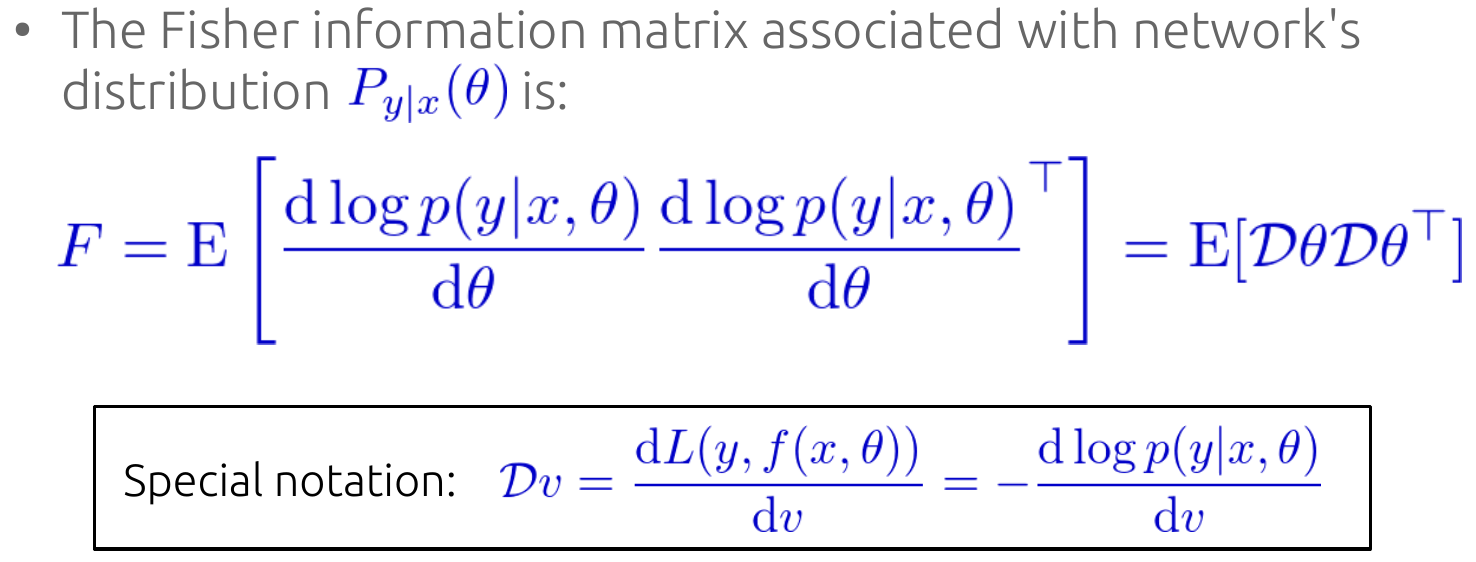
\includegraphics[scale=0.25]{fisher}
\end{figure}

\end{frame}

\section{Planning}
\frame{\tableofcontents[currentsection, hideothersubsections]}

\begin{frame}
\frametitle{How to control a robot from START to +1 (GOAL)?}
\begin{figure}
    \centering
    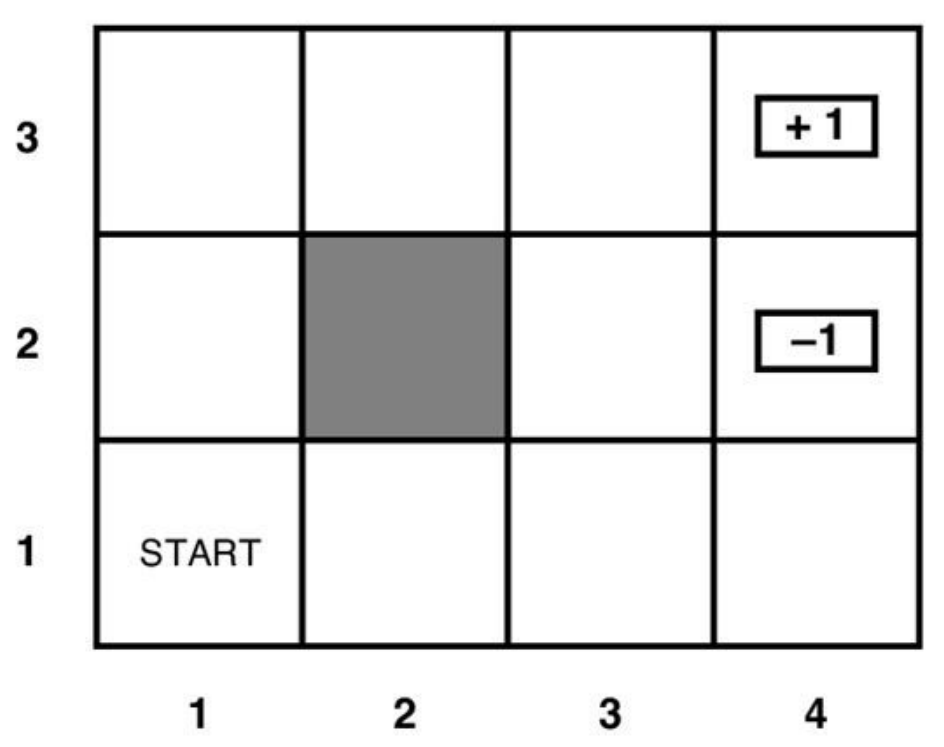
\includegraphics[scale=0.25]{grid_world_only}
\end{figure}
\pause

\begin{itemize}
  \item Wall following? right or left? who decides? \pause
  \item What if START can be in any grid? \pause
  \item What if actions are uncertain?
\end{itemize}
\end{frame}

\begin{frame}
\frametitle{How to control a robot from START to +1 (GOAL)?}
\begin{figure}
    \centering
    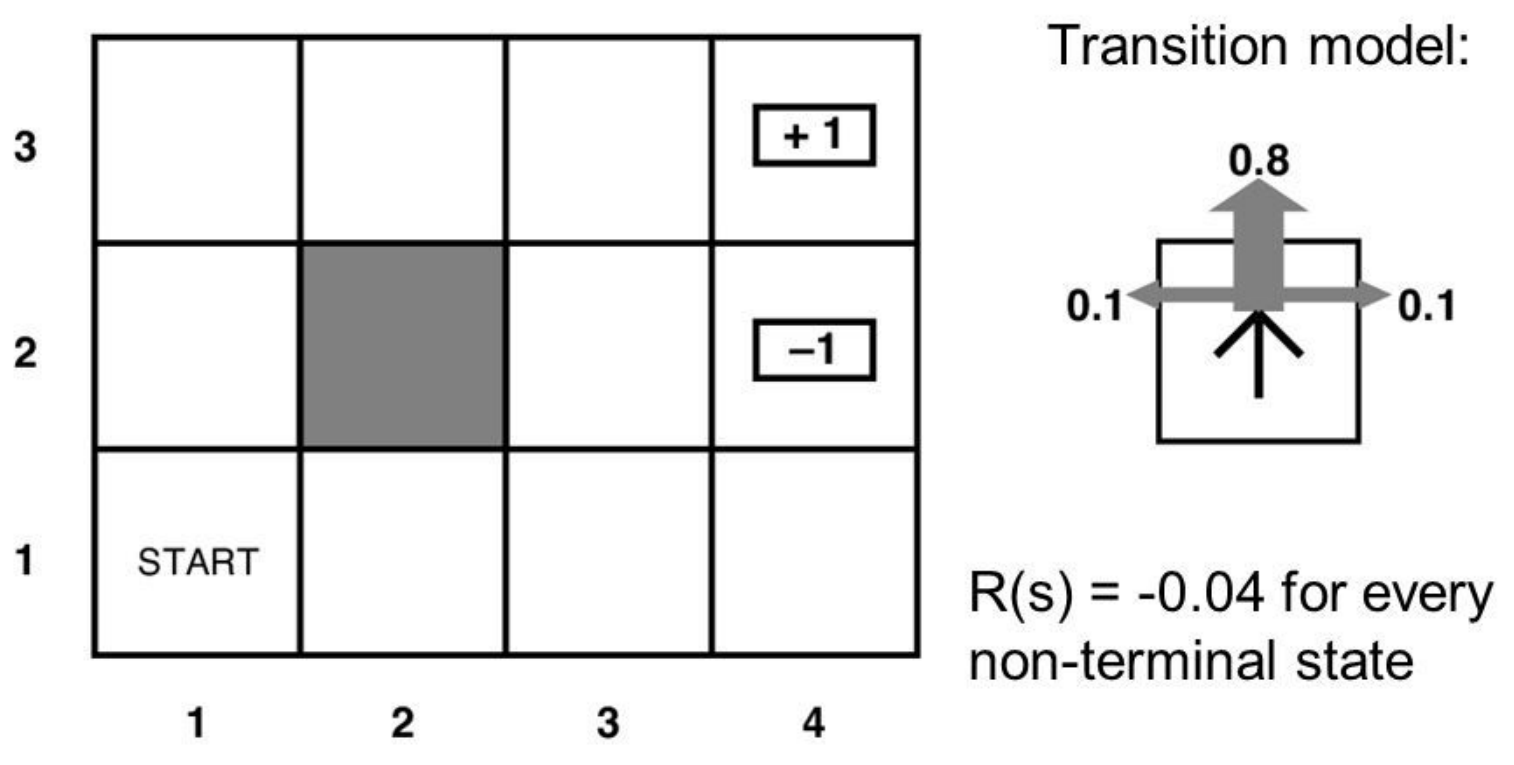
\includegraphics[scale=0.25]{grid_world_with_transition}
\end{figure}
\pause

\begin{itemize}
  \item Given environment model, one possible solution: \\
  \textbf{MDP planning}: sequential decision making under action uncertainty
\end{itemize}
\end{frame}

\begin{frame}
\frametitle{MDP: Markov Decision Process}
\begin{figure}
    \centering
    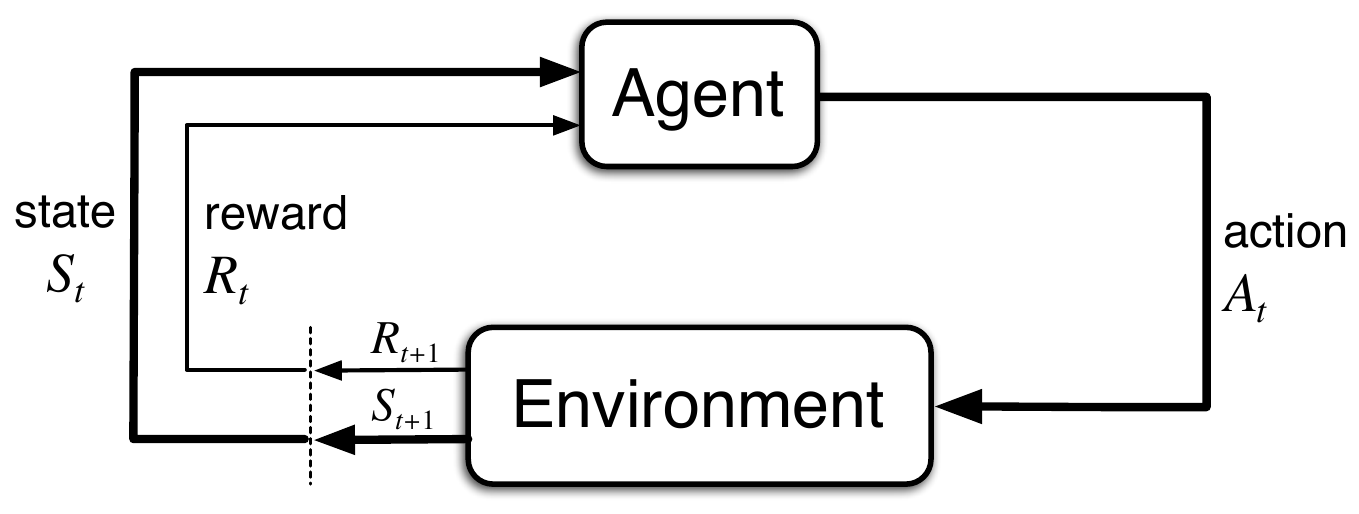
\includegraphics[scale=0.25]{agent_environment_rl_intro_p60}
\end{figure}
\pause
\begin{columns}
  \column{0.5\textwidth}
    $MDP = (S, A, T, R, \gamma)$ ... the model \pause
    \begin{itemize}
      \item $S$ is a set of states
      \item $A$ is a set of actions \pause
      \item $T(s,a,s') = P(s'| s, a)$ \\ is a transition function \pause
      \item $r:(s,a,s') \mapsto \mathbb{R}$ \\ is a reward function \pause
      \item $\gamma \in [0,1]$ is a discount factor
    \end{itemize}
    \pause
  \column{0.5\textwidth}
    \textbf{Agent's goal in MDP planning:}\\
    to maximize the return, $\mathcal{R}$,\\
    (i.e. the expected cumulative reward) \\
    \begin{align*}
      \mathcal{R}_t & = r_{t+1} + \gamma~r_{t+2} + \gamma^2~r_{t+3} + \ldots  \\
      & = \sum_{k=0}^{\infty} \gamma^k~r_{t+k+1}
    \end{align*}
\end{columns}
\end{frame}

\begin{frame}
\frametitle{MDP Planning: Value Function and Policy (Plan)}
\textbf{(State) value function:} the goodness of a state
\begin{align*}
V(s) & = \mathbb{E}[\mathcal{R}_t | S_t = s] \\
& = \mathbb{E} [r_{t+1} + \gamma~r_{t+2} + \gamma^2~r_{t+3} + \ldots | S_t = s] \\
& = \mathbb{E} [r_{t+1} + \gamma~ (r_{t+2} + \gamma~r_{t+3} + \ldots | S_t = s)] \\
& = \mathbb{E} [r_{t+1} + \gamma~ (\mathcal{R}_{t+1} | S_t = s)] \\
& = \mathbb{E} [r_{t+1} + \gamma~V(S_{t+1}| s)]
\end{align*}
\pause

\textbf{A policy (plan)} maps every state to an action, $\pi: s \mapsto a$, \\
generally, $\pi (a|s) = P[A_t = a|S_t = s]$
\end{frame}

\begin{frame}
\frametitle{MDP Planning: From Value Function To Policy}
$\pi = greedy(V)$ \\
Recall: the agents' goal is to maximize the expected cumulative return

\begin{columns}
  \column{0.5\textwidth}
    \begin{figure}
        \centering
        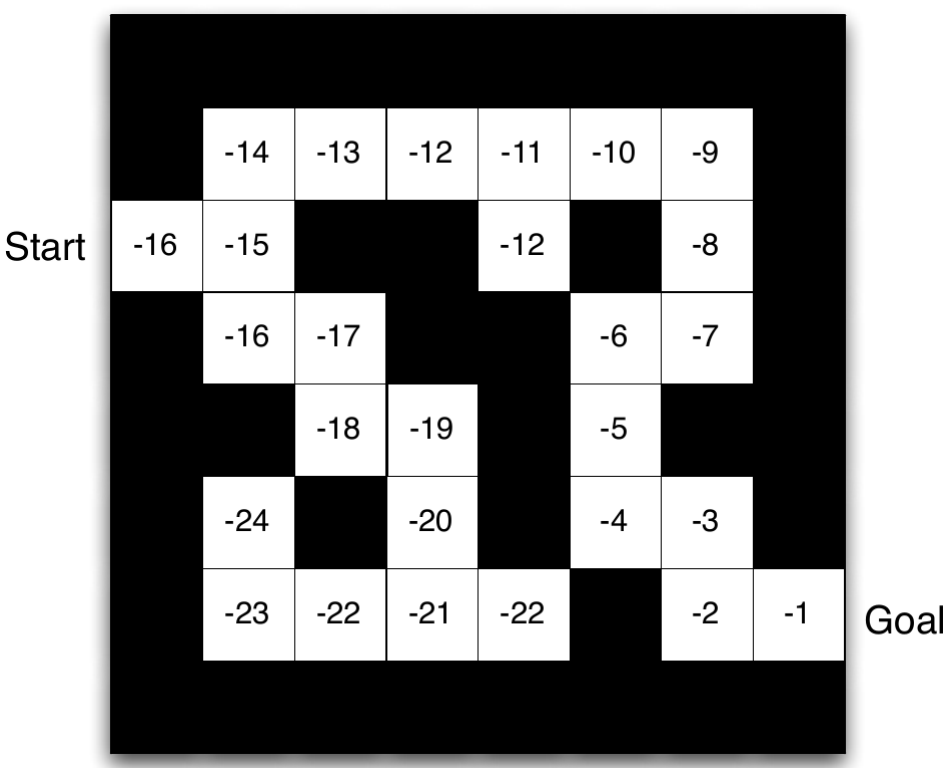
\includegraphics[scale=0.25]{value_function_example_silver_course}
        \caption{a (state) value function}
    \end{figure}

  \column{0.5\textwidth}
    \begin{figure}
        \centering
        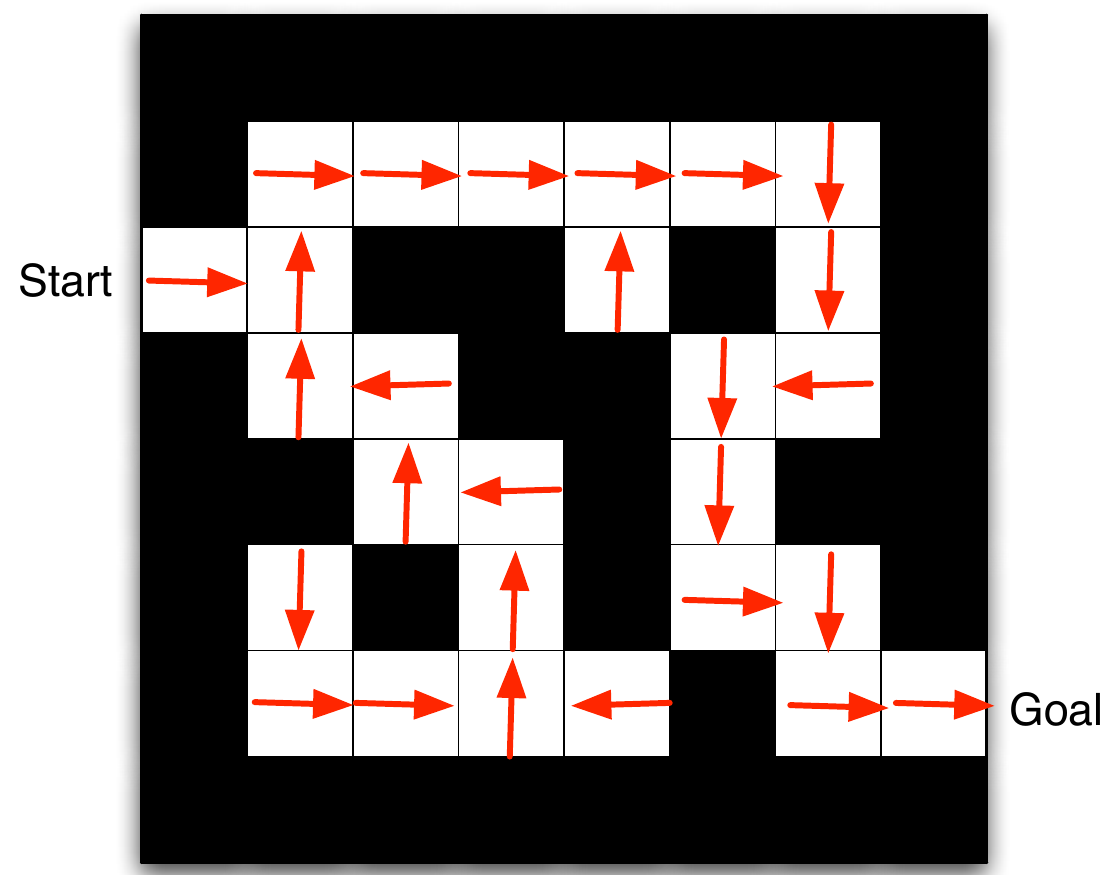
\includegraphics[scale=0.20]{policy_example_silver_course}
        \caption{a policy (plan)}
    \end{figure}
\end{columns}
\end{frame}

\begin{frame}
\frametitle{MDP Planning: Value Iteration (Dynamic Programming)}
\begin{figure}
    \centering
    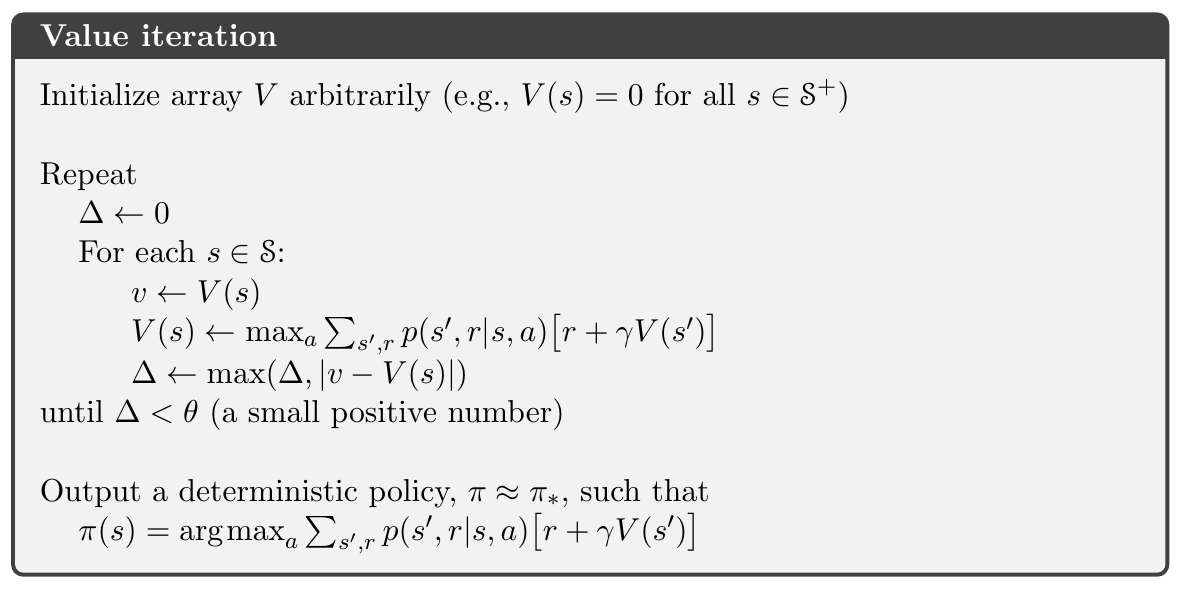
\includegraphics[scale=0.4]{value_iter_rl_intro_p92}
\end{figure}
\end{frame}

\begin{frame}
\frametitle{MDP Planning: Value Iteration Example}
\begin{figure}
    \centering
    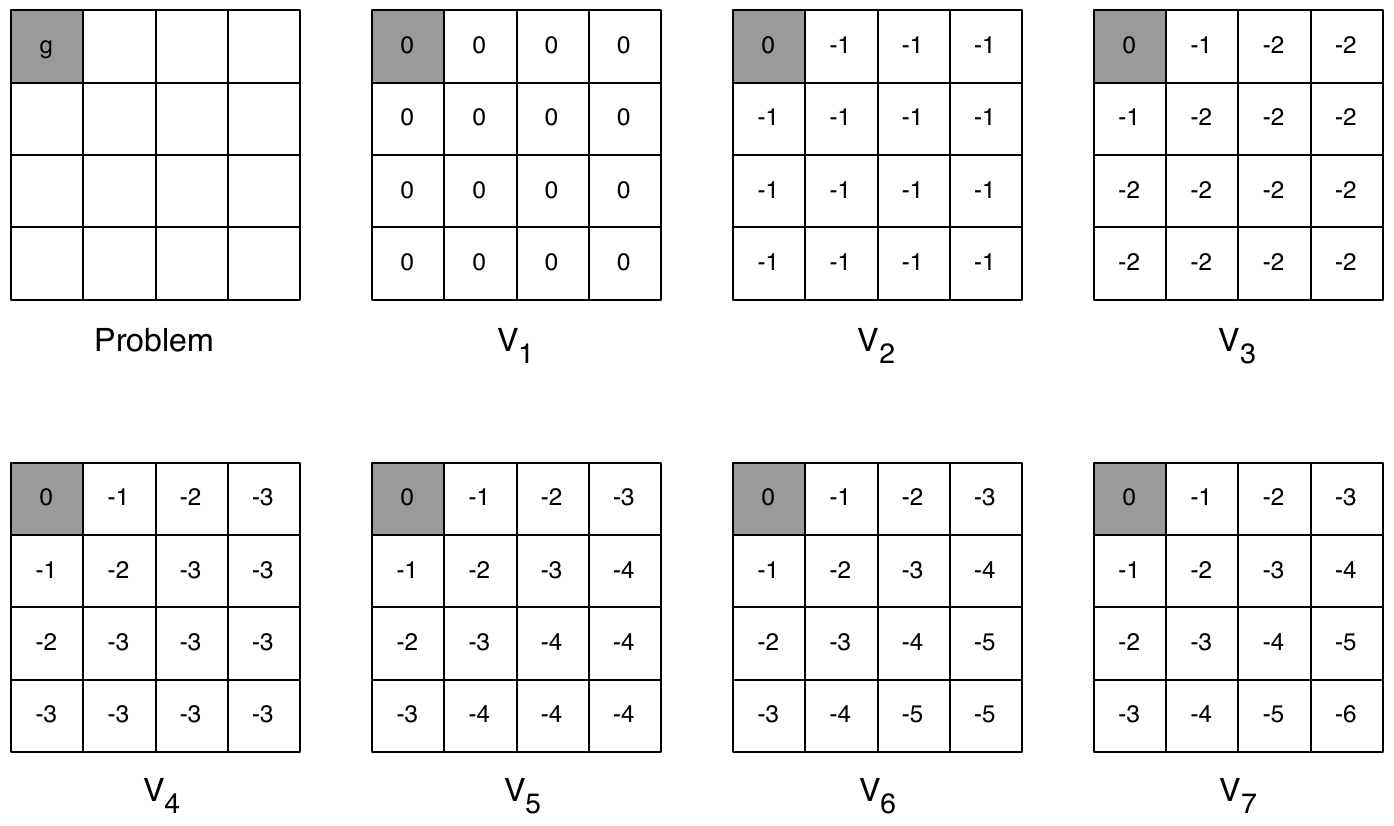
\includegraphics[scale=0.3]{value_iter_shortest_path_silver_course_2}
\end{figure}
\end{frame}

\begin{frame}
\frametitle{MDP Planning}
Iterations toward an optimal policy (plan)
\begin{figure}
    \centering
    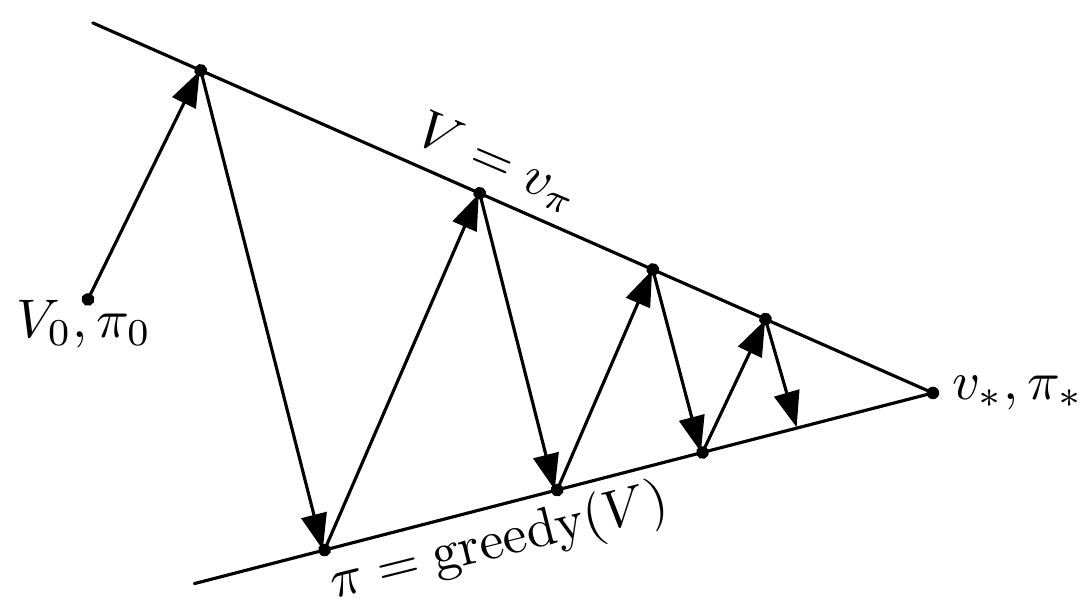
\includegraphics[scale=0.35]{gpi_rl_intro_p96}
\end{figure}
\end{frame}

\begin{frame}
\frametitle{MDP Planning}
\begin{figure}
    \centering
    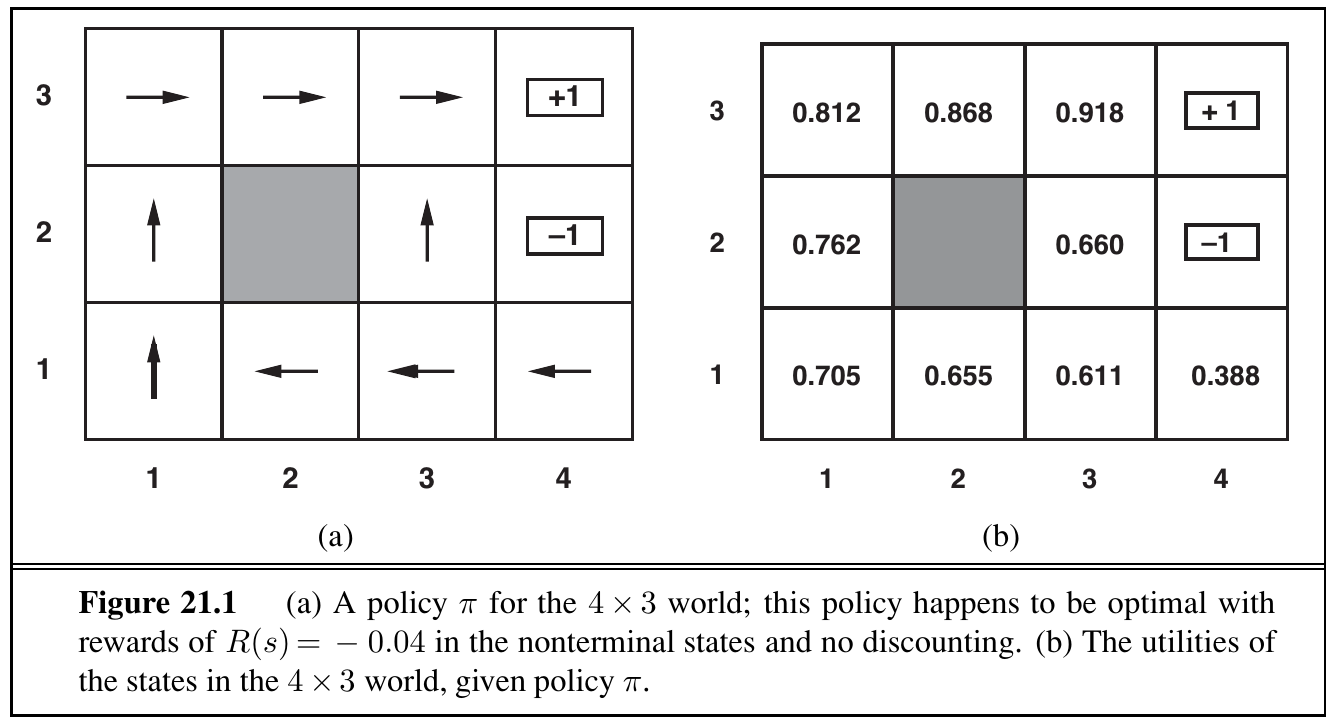
\includegraphics[scale=0.35]{policy_grid_world_aima_p832}
\end{figure}
\end{frame}
\section{Planning + Learning}
\frame{\tableofcontents[currentsection, hideothersubsections]}

\begin{frame}
\frametitle{Planning, Acting and Learning in MDP}
\begin{figure}
    \centering
    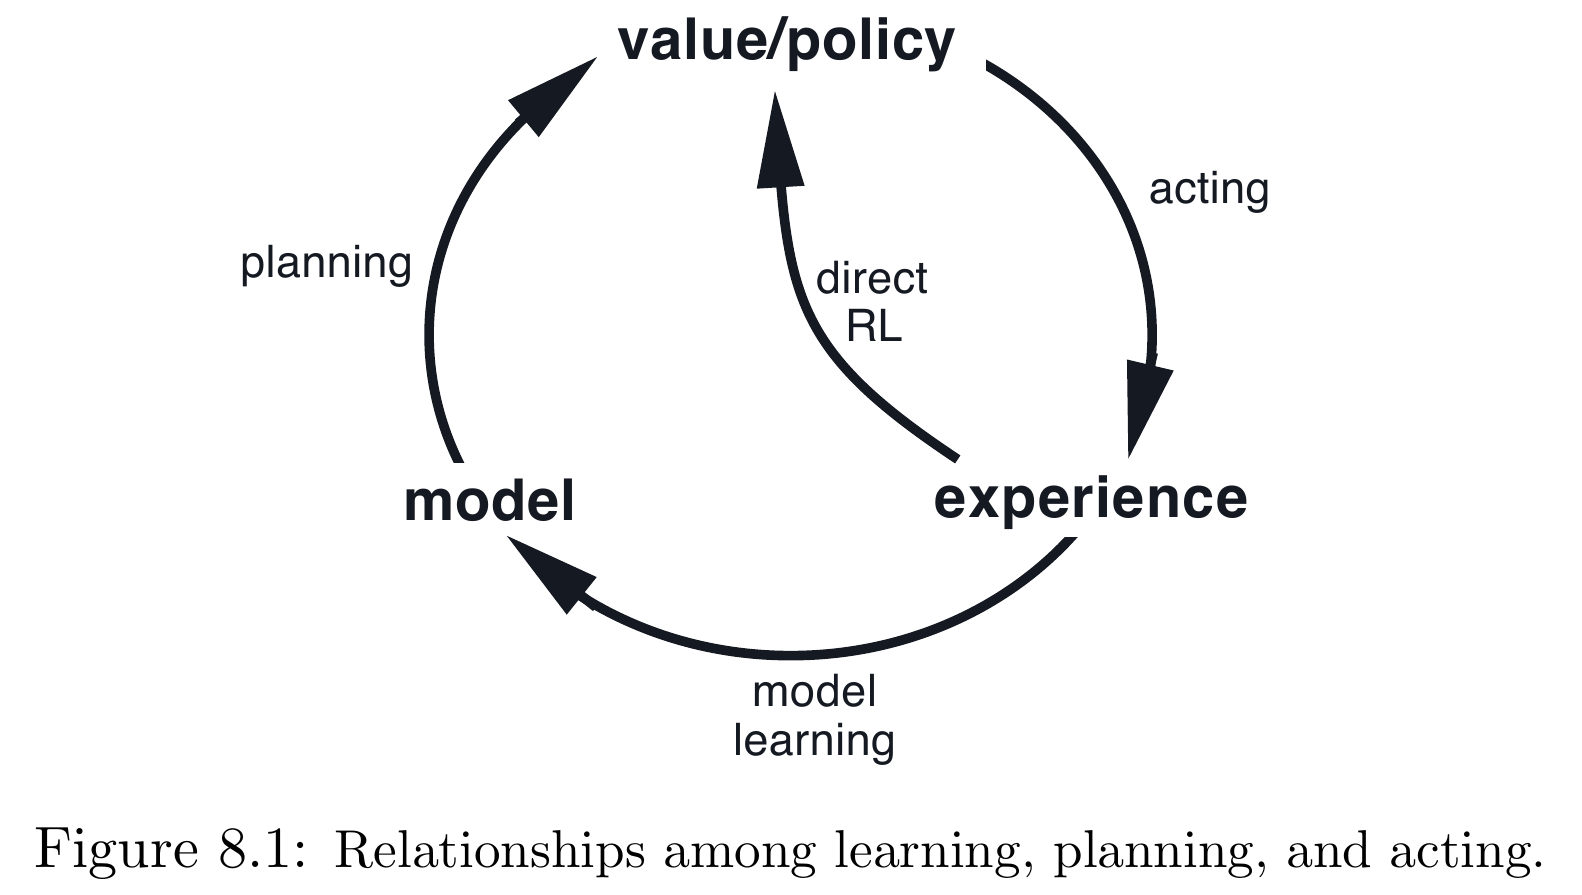
\includegraphics[scale=0.35]{learning_planning_acting_rl_intro_p176}
\end{figure}
\end{frame}

\begin{frame}
\frametitle{Planning vs direct Reinforcement Learning (Direct-RL)}
\begin{columns}
  \column{0.5\textwidth}
    \begin{figure}
        \centering
        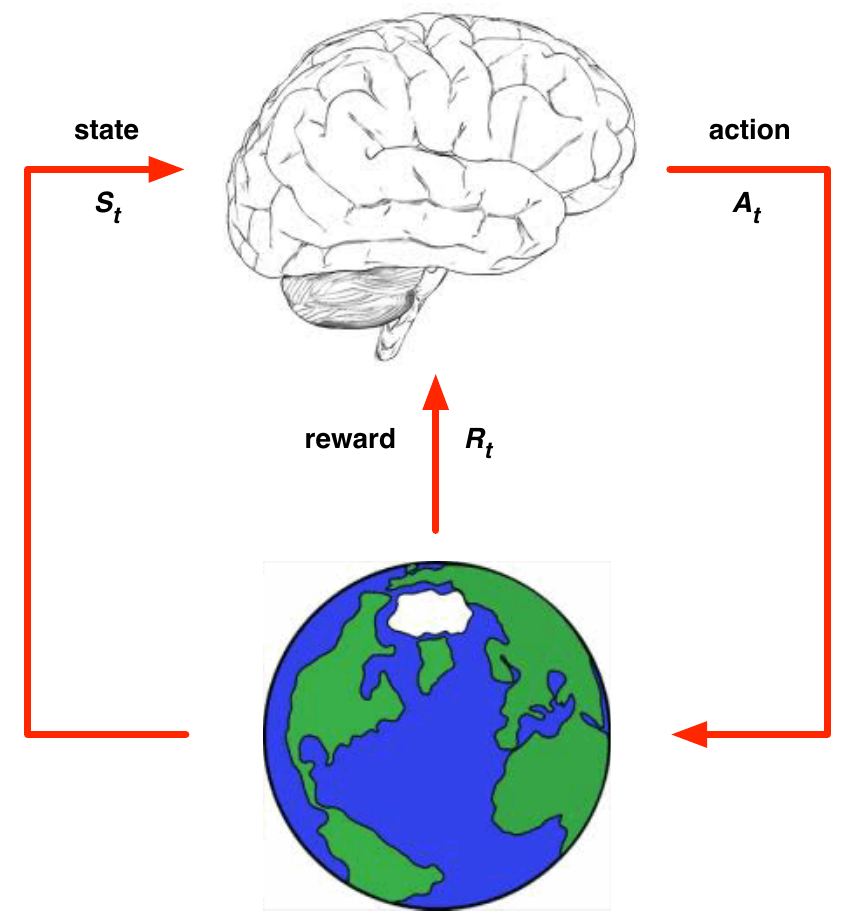
\includegraphics[scale=0.25]{model_based_silver_course}
        \caption{Planning uses a \textbf{model} env.}
    \end{figure}

  \column{0.5\textwidth}
    \begin{figure}
        \centering
        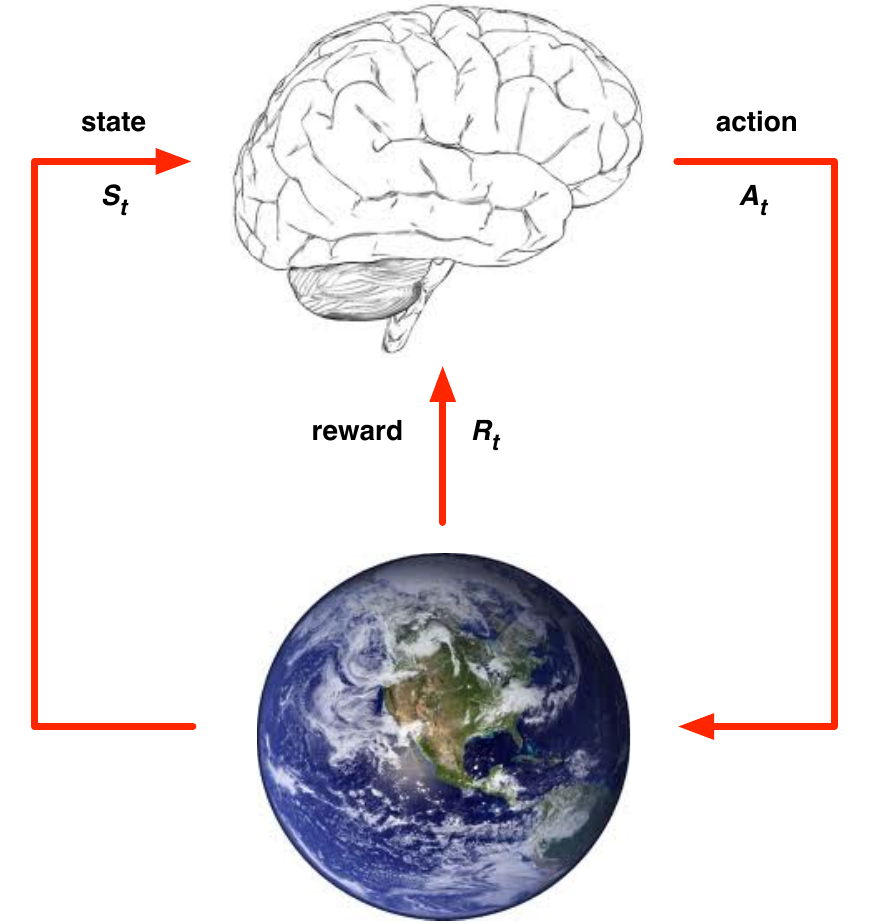
\includegraphics[scale=0.25]{model_free_silver_course}
        \caption{Direct-RL uses a \textbf{real} env.}
    \end{figure}
\end{columns}
\end{frame}

\begin{frame}
\frametitle{Planning vs direct Reinforcement Learning (Direct-RL)}
\begin{columns}
  \column{0.5\textwidth}
    \begin{figure}
        \centering
        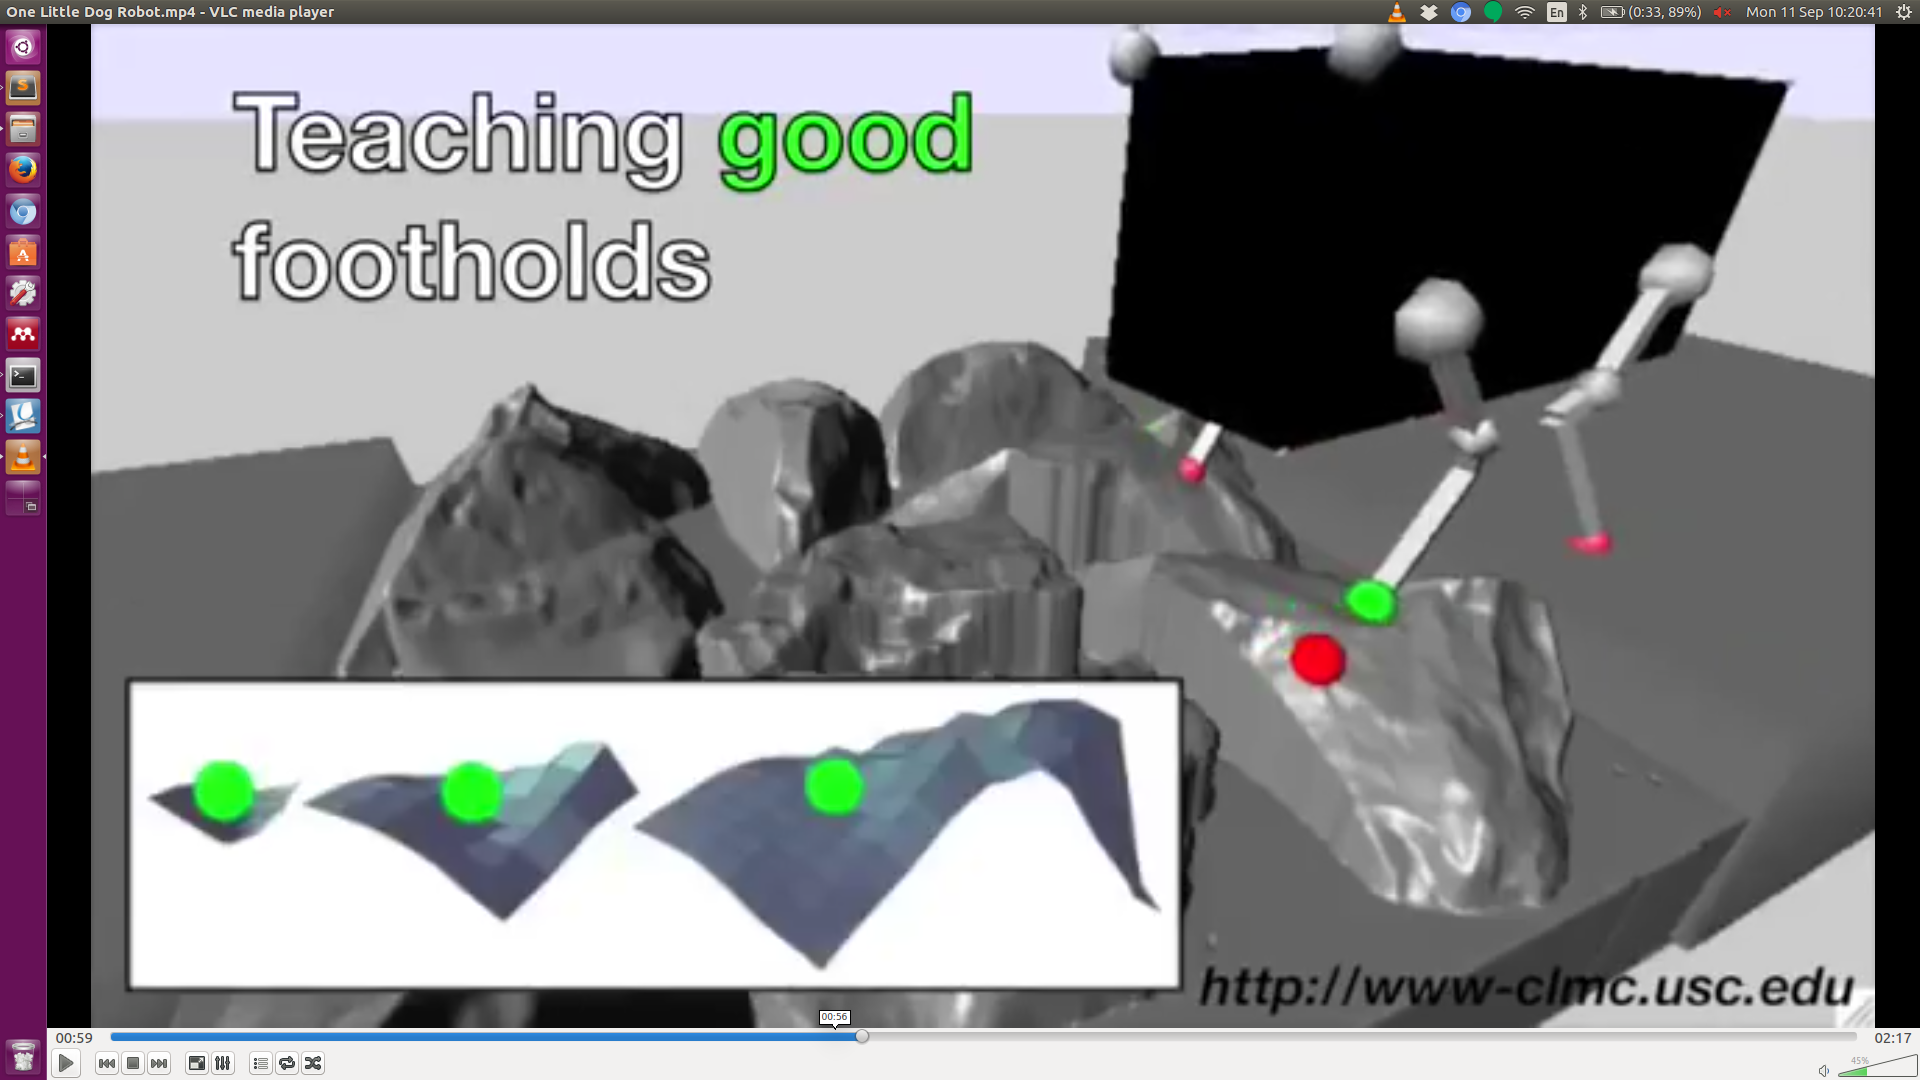
\includegraphics[scale=0.1]{little_dog_model_env}
        \caption{Planning uses a \textbf{model} env.}
    \end{figure}

  \column{0.5\textwidth}
    \begin{figure}
        \centering
        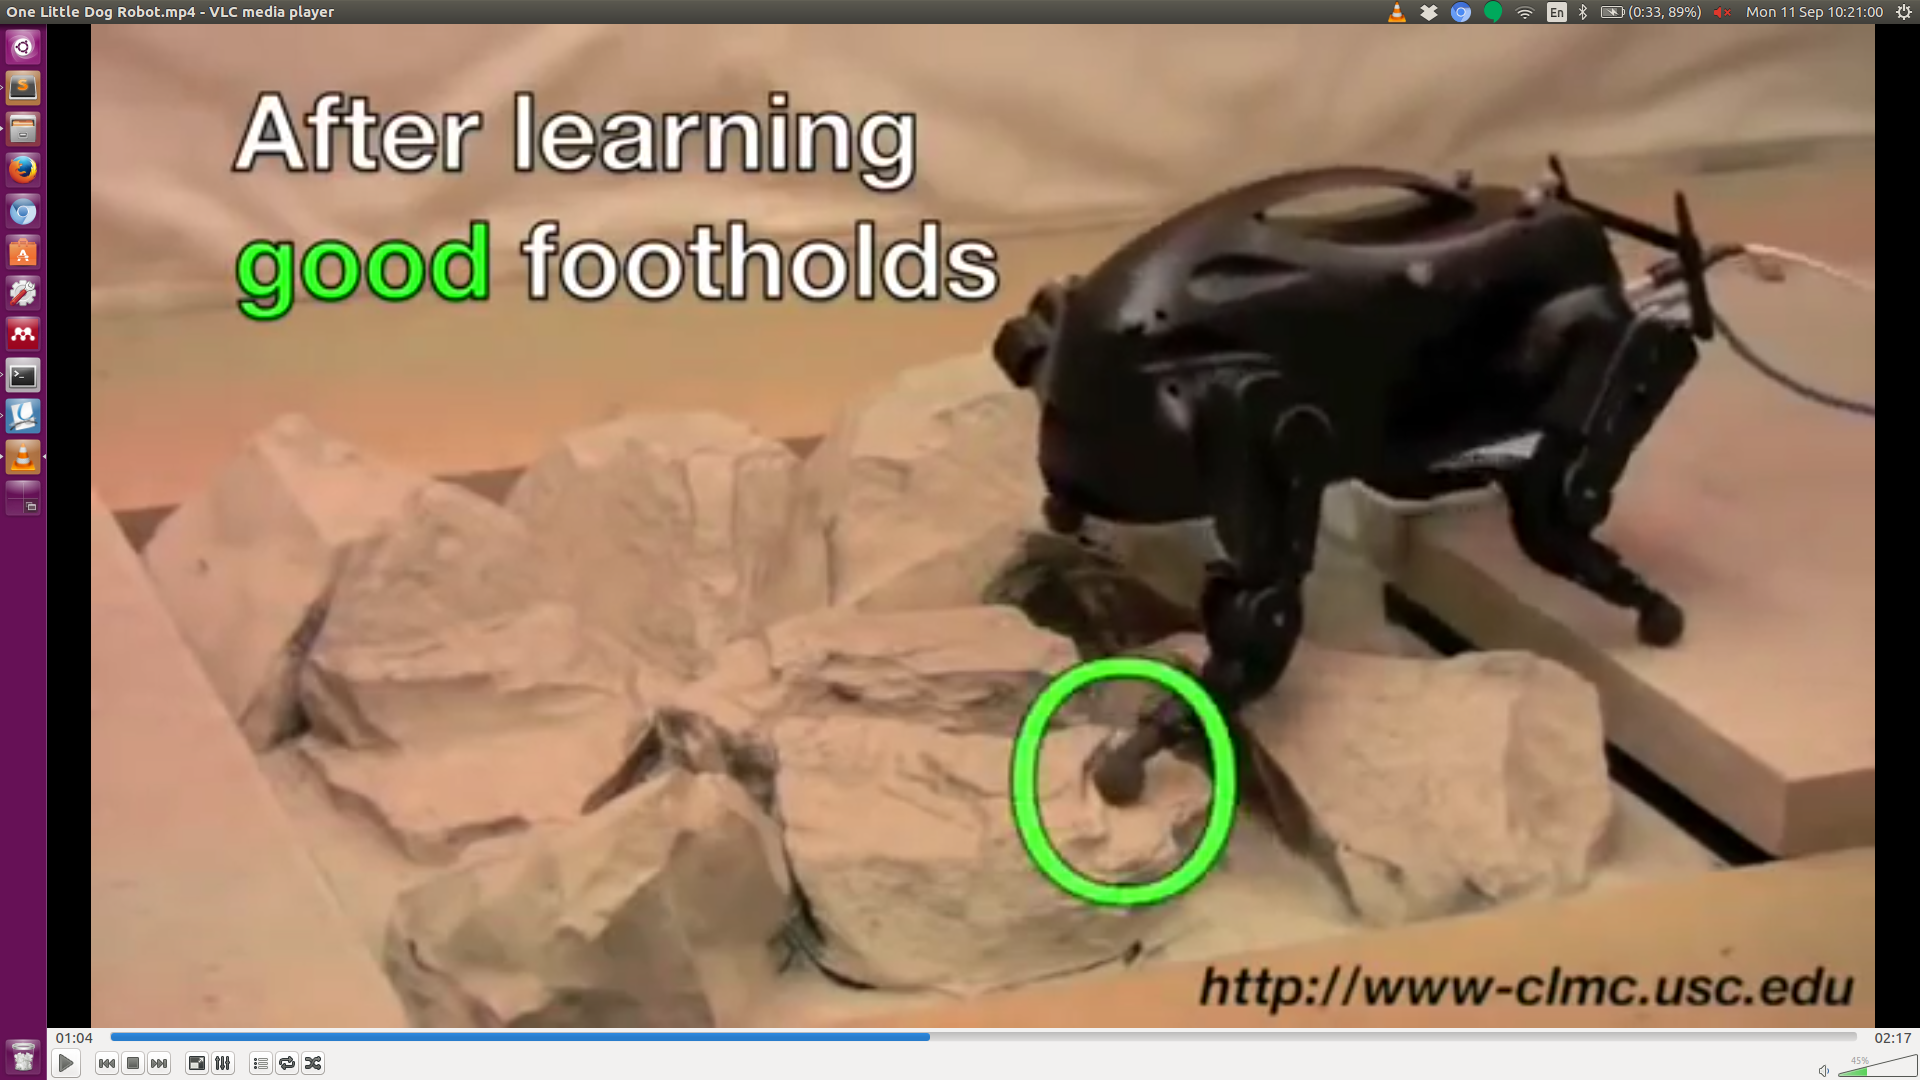
\includegraphics[scale=0.1]{little_dog_real_env}
        \caption{Direct-RL uses a \textbf{real} env.}
    \end{figure}
\end{columns}
\end{frame}

\begin{frame}
\frametitle{Q-learning for both planning and direct-RL}
\begin{figure}
    \centering
    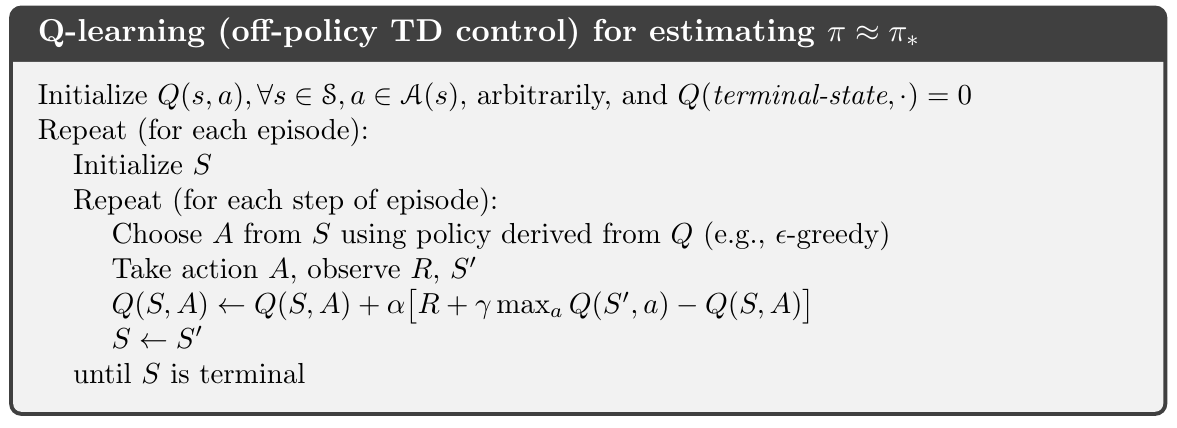
\includegraphics[scale=0.40]{q_learning_rl_intro_p142}
\end{figure}
\pause

\textbf{Action value-function} is the value of taking action $a$ in state $s$ \\
$Q(s,a) = \mathbb{E} [\sum_{k=0}^{\infty} \lambda^k~r_{t+k+1} | S_t = s, A_t = a]$\\
\noindent\rule{5cm}{0.4pt}\\
Note $Q:(s,a) \mapsto \mathbb{R}$,\\
\hspace{2mm} c.f $V: s \mapsto \mathbb{R}$
\pause

\end{frame}

\begin{frame}
\frametitle{Q-learning vs Value Iteration}
\begin{figure}
    \centering
    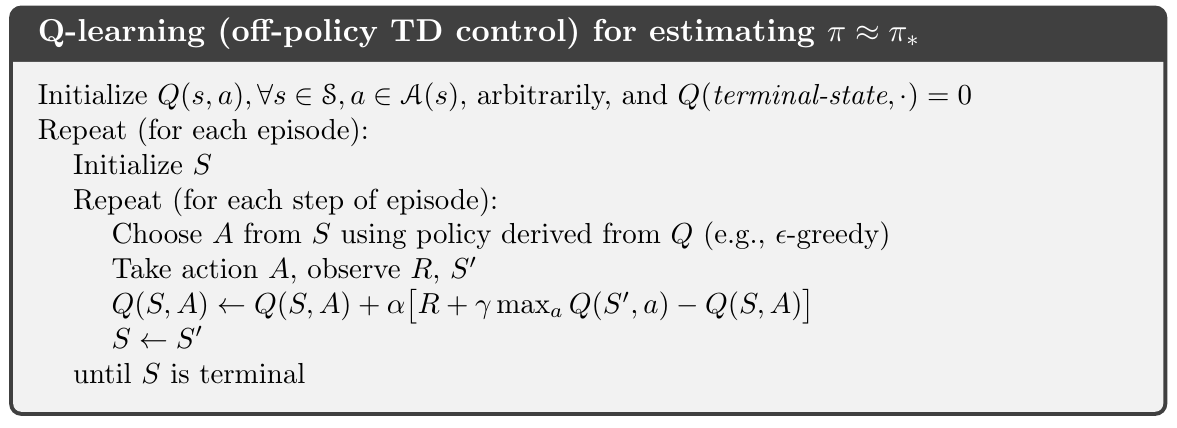
\includegraphics[scale=0.3]{q_learning_rl_intro_p142}
\end{figure}

\begin{figure}
    \centering
    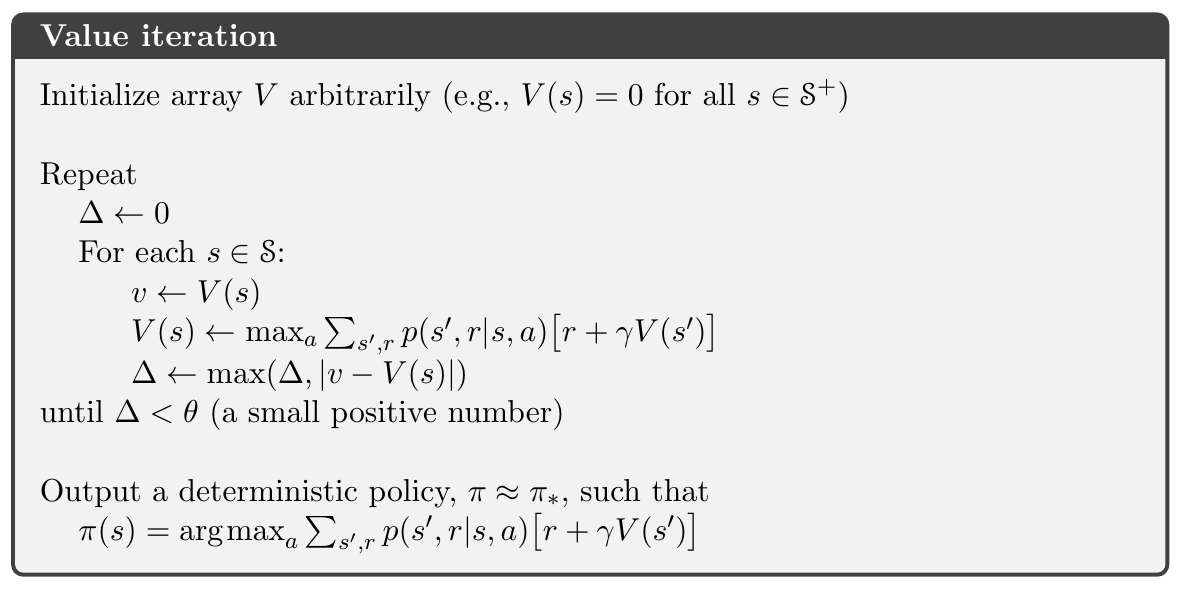
\includegraphics[scale=0.25]{value_iter_rl_intro_p92}
\end{figure}
\end{frame}

\begin{frame}
\frametitle{Dyna architecture}
\begin{figure}
    \centering
    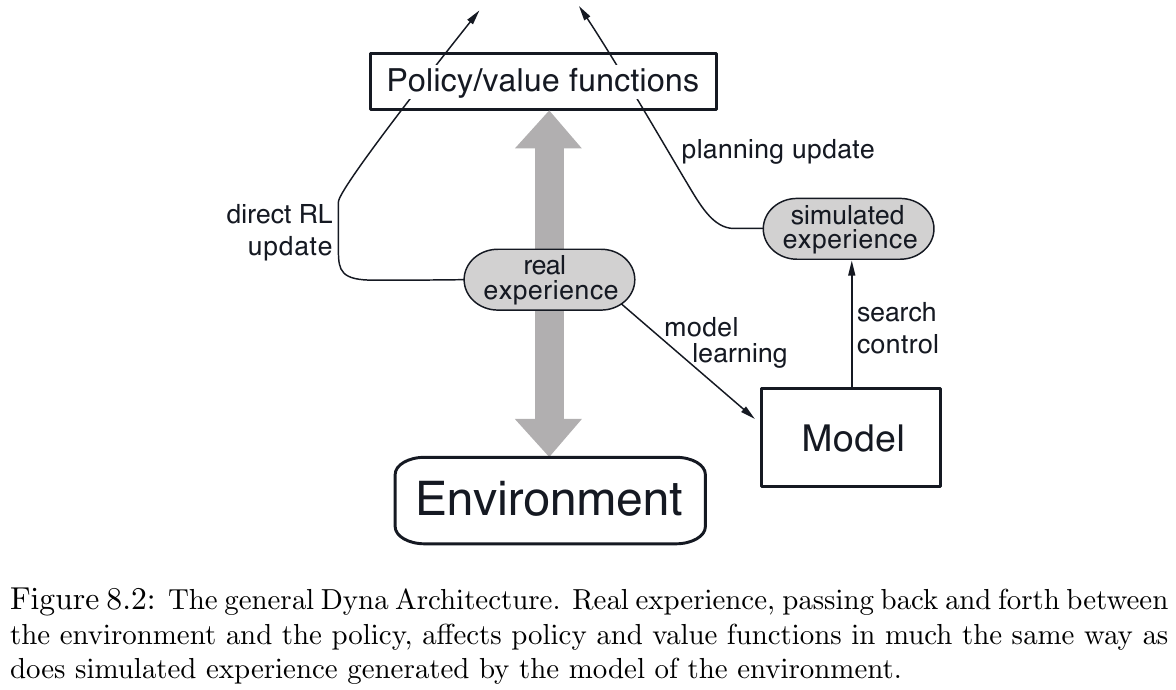
\includegraphics[scale=0.40]{dyna_rl_intro_p177}
\end{figure}
\end{frame}

\begin{frame}
\frametitle{Dyna algorithm}
\begin{figure}
    \centering
    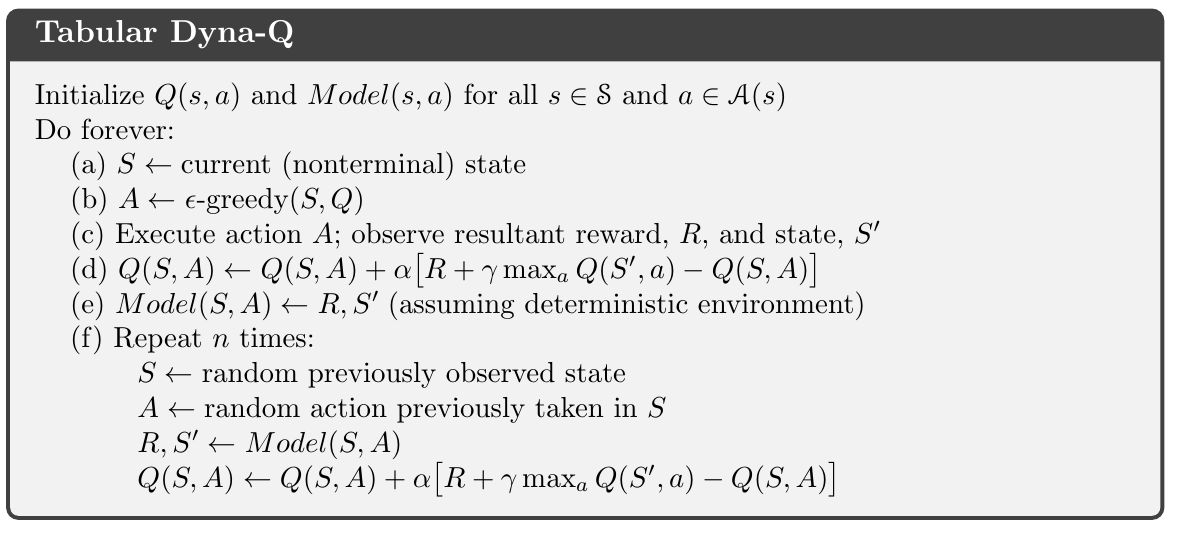
\includegraphics[scale=0.40]{dyna_algo_rl_intro_p178}
\end{figure}
\end{frame}

\begin{frame}
\frametitle{Dyna experiments}
\begin{figure}
    \centering
    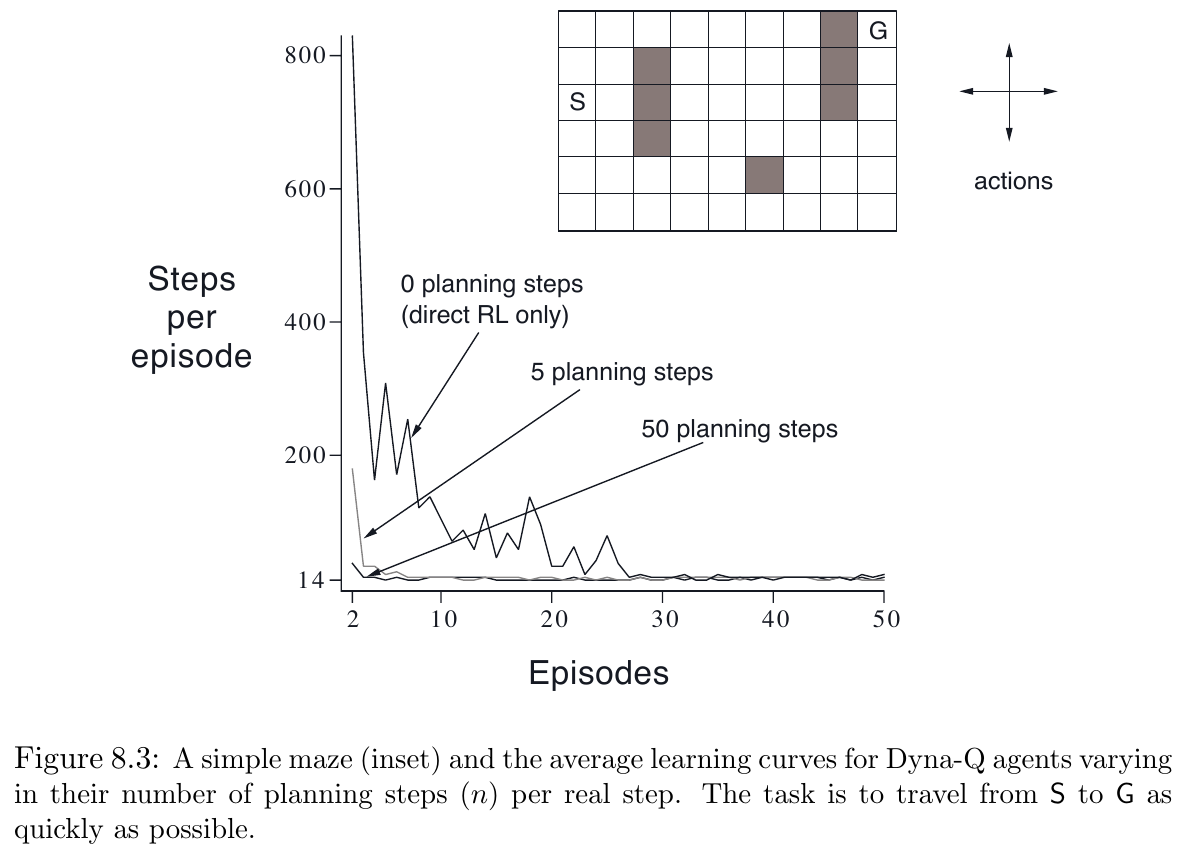
\includegraphics[scale=0.40]{dyna_plot_intro_p179}
\end{figure}
\end{frame}

\begin{frame}
\frametitle{Model learning as supervised and unsupervised learning}
\begin{figure}
    \centering
    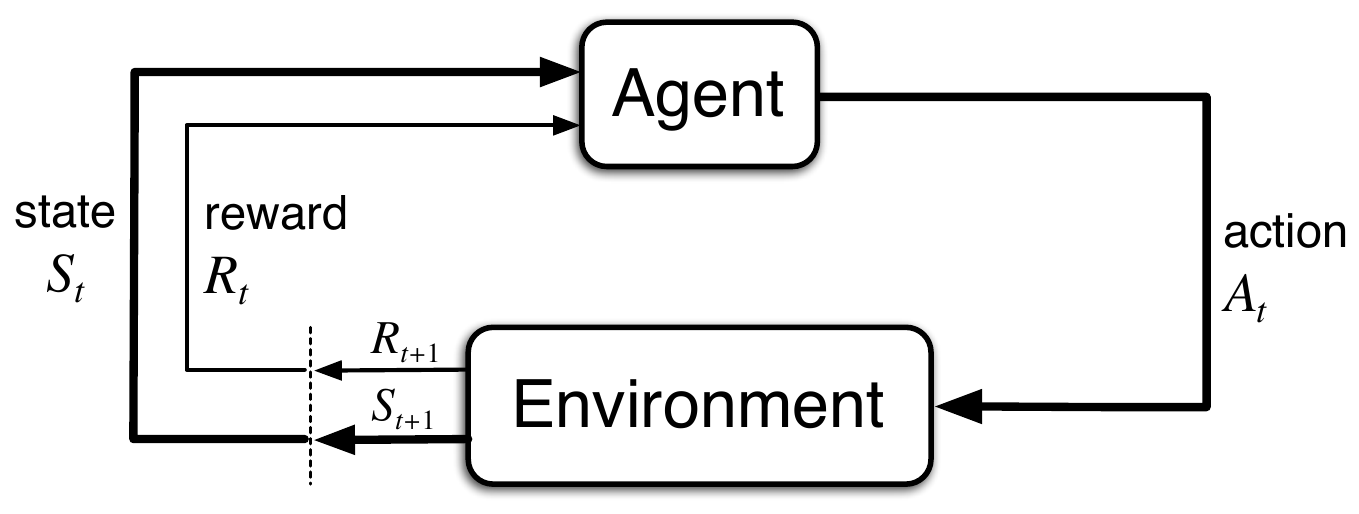
\includegraphics[scale=0.2]{agent_environment_rl_intro_p60}
\end{figure}

In model learning, \\
the goal is to estimate a model from experience, where:
$(S_1, A_1) \mapsto (S_2, R_2)$, \\
$(S_2, A_2) \mapsto (S_3, R_3)$,\\
\ldots,\\
$(S_{t-1}, A_{t-1}) \mapsto (S_t, R_t)$.
\vspace{2mm}
\pause

Thus, we have
\begin{itemize}
\item \textbf{regression} for the reward function, $(s, a) \mapsto r$
\item \textbf{density estimation} for the transition function, $(s, a) \mapsto s'$
\end{itemize}

\end{frame}

\begin{frame}
\frametitle{Changing (unstationary) Model}

Models may be incorrect because
\begin{itemize}
    \item the environment is stochastic and
    \item only a limited number of samples have been observed, or
    \item model was learned using function approximation
    \item the environment has changed
\end{itemize}

\end{frame}

\begin{frame}
\frametitle{Changing (unstationary) Model}

the Dyna agent with exploration bonus, Dyna-Q+,

% This
% agent keeps track for each state–action pair of how many time steps have elapsed since
% the pair was last tried in a real interaction with the environment. The more time that
% has elapsed, the greater (we might presume) the chance that the dynamics of this
% pair has changed and that the model of it is incorrect. To encourage behavior that
% tests long-untried actions, a special “bonus reward” is given on simulated experiences
% involving these actions. In particular, if the modeled reward for a transition is r,
% and the transition has not been tried in τ time steps, then planning backups are
% done as if that transition produced a reward of r + κ√
% τ , for some small κ.
\end{frame}


\section{Going further ...}
\frame{\tableofcontents[currentsection, hideothersubsections]}

\begin{frame}
\frametitle{Further questions:}
What if ...
\pause

\begin{itemize}
  \item $|S|$ and $|A|$ are big? $S$ and $A$ is continuous? \pause
  \begin{itemize}
    \item online planning that only plans from the current state
    \item sampling-based approaches, e.g. monte carlo planning
  \end{itemize}
  \pause

  \item states are partially observable? \pause
  \begin{itemize}
    \item formulate as Partially Observable MDP (POMDP)
  \end{itemize}
  \pause

  \item the (unknown) model changes during runtime? \pause
  \begin{itemize}
    \item keep learning and planning, improve the Dyna algorithm  :)
  \end{itemize}
  \pause

  \item want to study further? \pause
  \begin{itemize}
    \item see \cite{Sutton2017,Sugiyama2015,Poole2010,Russell2010,Szepesvari2010}
  \end{itemize}
\end{itemize}
\end{frame}
\section{Conclusions}
\frame{\tableofcontents[currentsection, hideothersubsections]}

\begin{frame}
\frametitle{Conclusions}
?
\end{frame}

\begin{frame}
\Huge{\centerline{Discussion time and thank you.}}
\end{frame}
\begin{frame} [allowframebreaks]
\frametitle{References}
{\tiny
\bibliographystyle{apacite}
\bibliography{ref}
}
\end{frame}

%%%%%%%%%%%%%%%%%%%%%%%%%%%%%%%%%%%%%%%%%%%%%%%%%%%%%%%%%%%%%%%%%%%%%%%%%%%%%%%

\end{document}
